\documentclass[12 pt]{article}
\usepackage{amsmath}
\usepackage{url}
\usepackage{graphicx}
\usepackage{setspace}
\usepackage{pgf}
\usepackage{tikz}
\usetikzlibrary{arrows,automata}
\usepackage[latin1]{inputenc}
\usepackage{verbatim}
\usepackage[margin=1.2in]{geometry}

%	\addtolength{\oddsidemargin}{-.5in}
%	\addtolength{\evensidemargin}{-.5in}
%	\addtolength{\textwidth}{0.75in}
%	\addtolength{\topmargin}{-1in}
%	\addtolength{\textheight}{1.75in}
\title{Final Year Project Interim Report\\ Predicting of Web 2.0 Thread Updates}
\author{U096883L Shawn Tan}
\date{}
\begin{document}
\doublespacing
\maketitle
\section{Introduction}
With the increasing number of Web 2.0 sites, sites with forums, or similar thread-based discussion features are extremely common. Data found on discussions like these provide useful feedback for content providers. As more users are involved with the content-generation process of these sites, maintaining an updated database of crawled content becomes increasingly difficult.


\begin{table}\label{table:web20}
	\makebox[\textwidth][c]{
	{\footnotesize
	\begin{tabular}{|l|c|c|c|c|c|c|c|c|c|c|}
		\hline
			\input{web20}
		\hline
	\end{tabular}
	}
	}
\caption{Features of popular Web 2.0 sites}
\end{table}

Looking at Table \ref{table:web20}, we find that many of the popular Web 2.0 sites have a comment feature. This suggests that content on the web is increasingly being created by users rather than content providers. While mining structured, curated content from sites like Amazon, for data like prices may be effective, data that can be obtained from user-generated content are of a different nature. One may be able to infer public sentiment about a given product, for example.

Web crawlers can be used to crawl sites for user comments and threads for postprocessing later. Web crawlers which maintain the `freshness' of a database of crawled content are known as incremental crawlers. Two tradeoffs these crawlers face cited by Yang et. al. 2009 \cite{Yang2009} are \emph{completeness} and \emph{timeliness}. \emph{Completeness} refers to the extent which the crawler fetches all the pages, without missing any pages. \emph{Timeliness} refers to the efficiency with which the crawler discovers and downloads newly created content. In this report, we will also discuss the \emph{freshness} of the local database, which refers to how new the extracted information is.

Let us define all such thread-based discussion styled sites as forums. Ideally, an incremental crawler of such user-generated content should be able to maintain a fresh and complete database of content of the forum that it is monitoring. A naive way to approach this would be to aggressively download these pages at a frequent rate. This, however, would (1) incur excessive costs when downloading un-updated pages, and (2) raise the possibility of the web master blocking the requester's IP address.

Thus, we need a strategy of revisiting pages that will reduce the cost of downloading unchanged pages, while at the same time downloading them as soon as possible after it's update.

\section{Related work}
In order to devise such a strategy, we need to predict how often any user may update the a page. Some work has been done to try to predict how often page content is updated, with the aim of scheduling download times in order to keep a local database fresh.

Many such works have used the Poisson distribution to model page updates. Coffman et. al. \cite{Coffman1997} analysed the theoretical aspects of doing this, showing that if the page change process is governed by a Poisson process $\lambda e^{-\lambda \mu}$, then accessing the page at intervals proportional to $\mu$ is optimal.

Cho and Garcia-Molina trace the change history of 720,000 web pages collected over 4 months, and showed empirically that the Poisson process model closely matches the update processes found in web pages\cite{Cho1999}. They then proposed different revisiting or refresh policies \cite{Cho2003,Garcia-molina2003} that attempt to maintain the freshness of the database.


The Poisson distribution were also used in Tan et. al. \cite{Tan2007} and Wolf et. al. \cite{Wolf2002}. %elaborate!!!!
However, the Poisson distribution is memoryless, and in experimental results due to Brewington and Cybenko \cite{Brian2000}, the behaviour of site updates are not. Moreover, these studies were not performed exclusively on online threads, where the behaviour of page updates may be very different from that of static pages.

Yang et. al. \cite{Yang2009}, attempted to resolve this by using the list structure of forum sites to infer a sitemap. With this, they reconstruct the full thread, and then use a linear-regression model to predict when the next update to the thread will arrive. %elaborate!!!

Online forums and bulletins have a logical, hierarchical structure in their layout, which typically alerts the user to thread updates by putting threads with new replies at the very top of the thread. However, this is not so for comments found on blog sites or discussion threads in an e-commerce site about a certain product.

These methods of estimating page updates either rely on previously gathered information about the page updates through repeated polling of the page, or through timestamps gathered from the individual posts. They have two shortfalls:

\begin{description}
	\item[Lack/Improperly formatted Timestamp Information] While most comment threads or forum sites tend to have timestamps, they often try to optimise readability. For example, timestamps of comments that were posted 8 months ago may be displayed as ``more than 4 months ago''.
	\item[Requires previous time series data]
		If the individual threads are treated independently of each other, a new thread (1 or 2 posts) would not have sufficient data to fit a Poisson model. Yang et. al. \cite{Yang2009} accounts for this by factoring into their regression model other threads with a similar recent history
\end{description}
The lack of these pieces of information may result in a poorer estimate, or no estimate at all. We argue, that the content within the posts of the thread should be important in predicting the thread updates.

For example, a thread in a technical forum about a Linux distribution may start out as a question. Subsequent questions that attempt to either clarify or expand on the original question may then be posted, resulting in a quick flurry of messages. Eventually, a more technically savvy user of the forum may come up with a solution, and the thread may eventually slow down after a series of messages thanking the problem solver. Suppose 10 days later, someone with a slight variation of the same problem posts on the thread again. A crawler solely on the age of the thread to determine its download rate of the thread may not update itself with the thread.

While there is little existing work using content to predict page updates, we will review some existing work related to analysing thread-based pages which we think will aid us in our efforts to do content-based prediction.

Kleinberg used Hidden Markov Models to predict ``bursts" in message arrival times \cite{Kleinberg2003}. In his running example, he used email messages, and used time between messages to estimate the states that produced the sequence. While the model may be able to predict what the state is for the next time interval, it does so using the history of message arrival times, and does not take into account the content within the messages themselves.

One work related to evaluating content on threads relates to finding out linkages between forum posts using lexical chaining \cite{Wang2011}. They proposed a method to link posts using the tokens in the posts called $Chainer_{SV}$. While they do analyse the content of the individual posts, the paper does not make any prediction with regards to newer posts.



\section{Possible Approaches}

\subsection{Hidden Markov Models}
We could modify Kleinberg's use of HMMs to detect bursts in his email stream \cite{Kleinberg2003}. Instead of using time differences as the observations we would use the content of the pages.

If we assume that a thread is governed by a set of discrete states, say `Active'($q_0$) and `Inactive'($q_1$), and each of these states stochastically transit from one to the other or back to itself. The states also produces certain observable characteristics $\mathbf{z}$, with probability $P(\mathbf{z}|q)$ where $q$ is a state. In the case of our thread content, possible observations include:
\begin{description}
	\item[Average length of a post] The average length of a post may be indicative of the activity on the thread. An active discussion may result in long posts to explain steps, or to elaborate arguments.
	\item[Word frequencies] Certain words may appear often in an active or inactive thread. A thread that may be transitioning toward an `Inactive' state may be more likely to have higher occurences of `Thank you', for example.
	\item[Time between posts] We could include the average time differences, since they are indicative of a thread that is still relatively active.
\end{description}
Since new posts are more likely to be influenced by more recent posts, a form of weighted importance should be introduced, giving the later posts greater influence on the prediction.

\subsubsection{Lexical Chaining}
One way to leverage the content in the thread might be to look at the post linkage structure. Lexical chaining gives a numerical relationship between theach post in the thread. Analysing the time between these posts and the lexical chains, we may be able to predict, given the posts in the thread, when the next post may arrive.

With these observations, the states that produce them, and the transitions between the states, given a thread, we may be able to produce a sequence of states that are highly likely to generate the observations. If we assume a certain rate of updates in each state, we would be able to calculate the expected interval between the last post and a future post.


\section{Work in progress}
\subsection{Extracting data}
In order to determine if there is a relationship between the lexical chains in a thread and the arrival of the next post, we need to collect data from a popular forum with fairly long threads. We chose \url{http://forum.hardwarezone.com.sg} as our data set.

We have been scraping the Hardwarezone forums daily in order to build a database of threads and their User, Timestamp, Content tuples. The scraped data from the forums are still currently in their raw HTML format. We need to extract the feature vectors in order to train the HMM.
\subsection{Implementation of baseline}
We intend to implement the algorithm used in Yang et. al. \cite{Yang2009}, as a baseline to evaluate our system. However, since the algorithm uses the overall sitemap as additional information, only the linear regression model used to predict future incoming posts will be used. We will also use an SVM, trained using discretised time intervals and the extracted feature vectors.

\subsection{Modeling of threads}
Modelling the problem as an HMM problem requires us to define a set of possible states that emmit the observable features on the thread. This requires more in-depth understanding of how users behave on a forum. Once this is done, a sets of training data would have to be annotated as produced by the different states. We also need to train the transitions between the states.

The feature vector to be extracted from the current thread would also need to be defined. More study must be done to see the most effective way to weigh the features extracted per post to make the more recent posts more `important' in the extracted feature vector.

\subsubsection{Initial model}
\begin{figure}\label{sleepcycle}
\makebox[\textwidth][c]{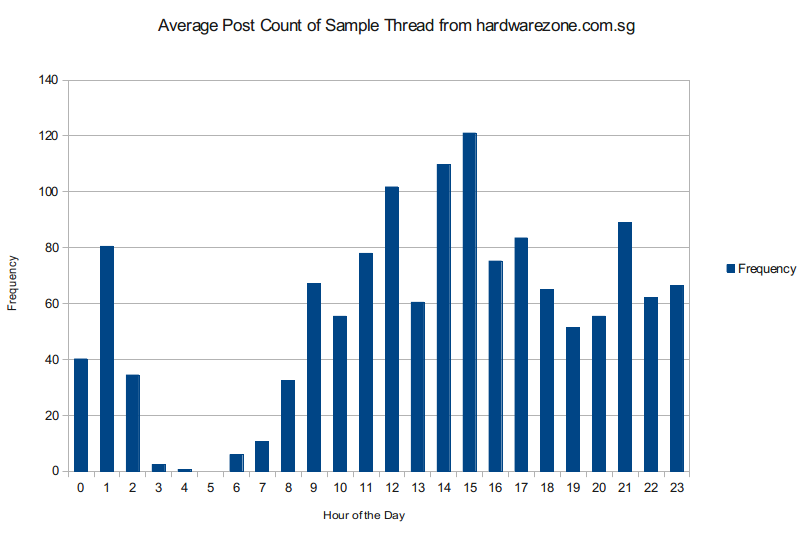
\includegraphics[scale=0.5]{threadfreq.png}}
\caption{The post frequency of a thread from forums.hardwarezone.com.sg shows a pattern cycle of the forum's users.}
\end{figure}
From our initial analysis of the extracted data from the Hardwarezone forums, we have made the following observations about non-sticky threads in the forum:
\begin{enumerate}
	\item There are threads that are very short-lived, and some that are long lived. This is largely dependent on the thread content. For example, a user looking to buy/sell a product that no one has an interest in.
	\item The long-lived threads typically have a pattern to the frequency of postings. A high frequency of posts are seen around lunch time (12-3 PM) and another spike is seen during the night at 9 PM. (Figure \ref{sleepcycle}). It is yet to be determined if this type of cycle is site-wide or thread-specific.
\end{enumerate}
We propose that the thread is governed by a probabilistic automata. Our initial model aims to incorporate these observations. A new thread (represented by $q_0$) which only has one post, may transition into either an active or inactive state (represented by $q_A,q_I$ respectively). We define active here as threads with high post frequency, and inactive threads as posts with low post frequency. Since our observations show that threads have different levels of post frequencies due to usage patterns consistent with user's sleep cycles, we use four states in total to represent the state of a thread with more than 2 posts, a `day' state and a `night' state (represented by $q_D,q_N$). These four states form a clique. Each of these states produce a set of observations that we can use to identify the state that a thread is in.

The intuition behind this is the fact that active threads can transition to an inactive state, but the presence of a new post is able to spark off a new discussion within the thread, causing it to be an active thread again.

The graphical representation of this automata is seen in Figure \ref{spaceship}.


\begin{figure}[H]
	\begin{center}
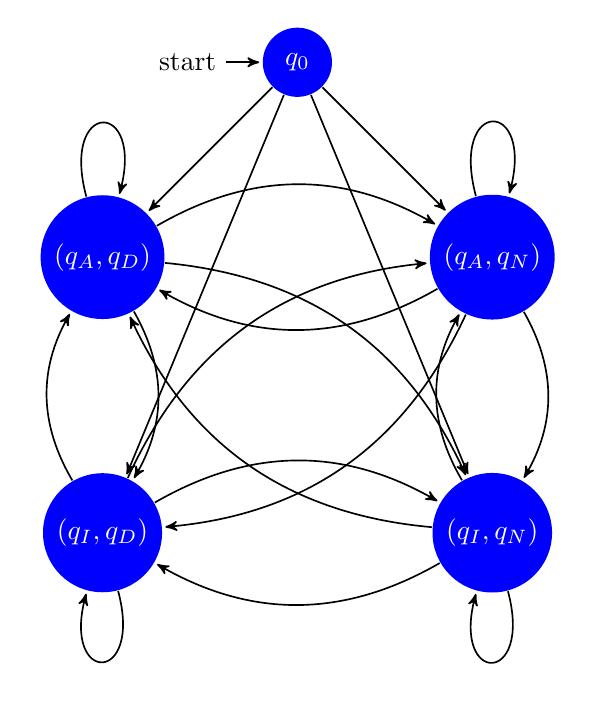
\begin{tikzpicture}[->,>=stealth',shorten >=1pt,auto,node distance=3.5cm,
                    semithick]
  \tikzstyle{every state}=[fill=blue,draw=none,text=white]

  \node[initial,state] (q0)                    {$q_0$};
  \node[state]         (AD) [below left of=q0] {$(q_A,q_D)$};
  \node[state]         (AN) [below right of=q0] {$(q_A,q_N)$};
  \node[state]         (ID) [below of=AD] {$(q_I,q_D)$};
  \node[state]         (IN) [below of=AN] {$(q_I,q_N)$};

  \path (q0) edge              node {} (AD)
 			 edge 			   node {} (AN)
			 edge              node {} (ID)
			 edge 			   node {} (IN)
		(AD) edge [loop above] node {}(AD)
			 edge [bend left]  node {}(AN)
			 edge [bend left]  node {}(ID)
			 edge [bend left]  node {}(IN)
		(AN) edge [bend left]  node {}(AD)
			 edge [loop above] node {}(AN)
			 edge [bend left]  node {}(ID)
			 edge [bend left]  node {}(IN)
		(ID) edge [bend left]  node {}(AD)
			 edge [bend left]  node {}(AN)
			 edge [loop below] node {}(ID)
			 edge [bend left]  node {}(IN)
		(IN) edge [bend left]  node {}(AD)
			 edge [bend left]  node {}(AN)
			 edge [bend left]  node {}(ID)
			 edge [loop below] node {}(IN);
\end{tikzpicture}

\end{center}
	\caption{Preliminary modelling of a thread as a probabilistic automaton}\label{spaceship}
\end{figure}
Our initial collection of data to identify changes in state for active threads to inactive threads do not show any observable patterns (See Figure \ref{nothing}). More data has to be collected and analysed before conclusions can be made. Statistics of textual content, along with data for a more complete set of threads may provide some insight to their behaviour.

\section{Conclusion}
A lot remains to be done over the next half of the academic year. More data for more sites with thread-based comment systems have to be collected in order to come up with a more general model. The baseline algorithms have to be implemented in order to perform evaluation. Most importantly, our algorithm has to be implemented and then evaluated against the baseline.


\begin{figure}[h]
	\makebox[\textwidth][c]{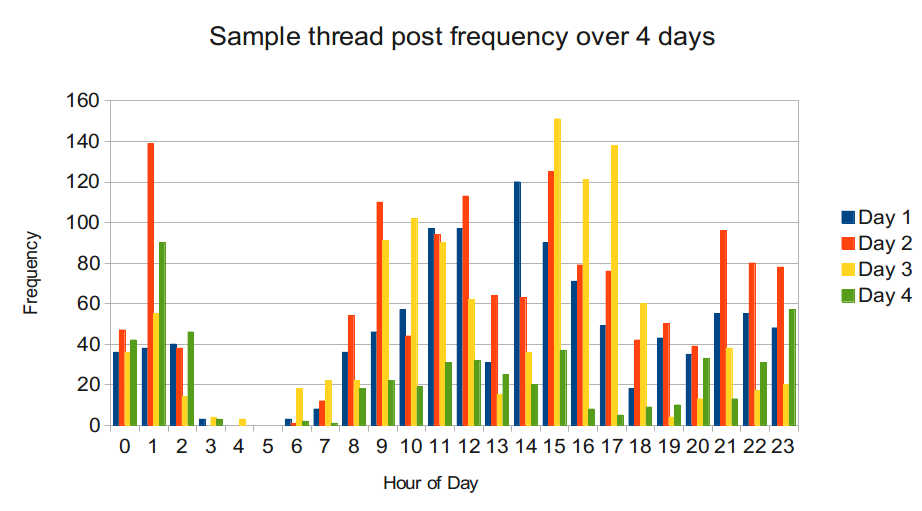
\includegraphics[scale=0.5]{4daysthreadfreq.png}}
	\caption{No conclusion to be drawn for post frequencies over four days.}\label{nothing}

\end{figure}




%\begin{figure}
%	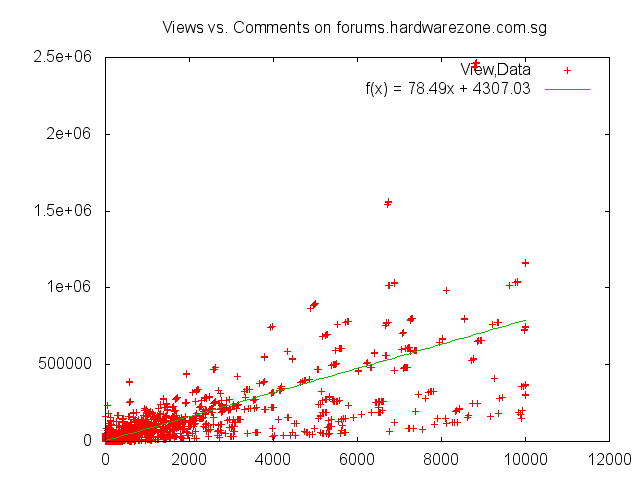
\includegraphics[scale=0.5]{view-comment.png}
%	\caption{Linear fit of Views vs Comments from forum.hardwarezone.com.sg}
%\end{figure}

\bibliographystyle{acm}
\bibliography{report}
\end{document}
